\chapter{Исследовательский раздел}
В данном разделе будет проведено функциональное тестирование разработанного программного обеспечения и измерение временных характеристик каждого из реалтзованных алгоритмов.

В этой лабораторной работе будет использована библиотека Google Test и стандратная библиотека C++. 

\section{Технические характеристики}

Технические характеристики устройства, на котором проводилось исследование:

\begin{itemize}
    \item Процессор: AMD Ryzen 2700 4.00GHz \cite{ryzen}.
    \item Оперативная память: 16GiB.
    \item Операционная система: Linux Kernel 5.14.8 \cite{kernel}.
\end{itemize}

Исследование проводилось на стационарном компьютере, включенном в сеть электропитания. Во время проведения эксперимента компьютер был нагружен только работой ядра линукса, системных служб и терминала. 

\section{Тестирование}

В данном разделе приведена таблица с тестовыми данными (таблица \ref{tab:tests}).



\begin{table}[ht]
  \caption{Таблица с тестами}
 \begin{tabular}{|*3{>{\renewcommand{\arraystretch}{1}}c|}}
\hline
\textbf{Матрица №1} & \textbf{Матрица №2} & \textbf{Ожидаемый результат}\\
\hline
$\left[ \begin{array}{c} 2 \end{array}\right]$ & $\left[ \begin{array}{c} 2  \end{array}\right]$ & 
$\left[ \begin{array}{c} 4 \end{array}\right]$\\
\hline
$\left[ \begin{array}{cc} 0.1 & 0.5 \end{array}\right]$ & $\left[ \begin{array}{c} 0.01 \\ 0.2  \end{array}\right]$ & 
$\left[ \begin{a rray}{cc} 0.001 & 0.02  \\ 0.005 & 0.1 \end{array}\right]$\\
\hline
$\left[ \begin{array}{ccc} 0.1 & 0.5 & 0.6 \\ 0.5 & 0.1 & 0.6 \end{array}\right]$ & $\left[ \begin{array}{cc} 0.01 & 0.9 \\ 0.2 & 0.8 \\ 0.3 & 0.4  \end{array}\right]$ & 
$\left[ \begin{array}{ccc} 0.281 & 0.73 \\ 0.205 & 0.77 \end{array}\right]$\\
\hline
\end{tabular}
\label{tab:tests}
\end{table}
Во время проведения функционального тестирования, полученные тестовые данные полностью совпали с ожидаемыми --- тестирование прошло успешно. 

\section{Временные характеристики}
Время выполнения алгоритмов было найдено при помощи библиотеки Google Benchmark \cite{google_benchmark}. 
Результаты измерения времени (в наносекнудах) были зафиксированы в Таблице \ref{tab:benchmark}.

Для измерения временных характеристик были выбраны две квадратные матрицы размерностью от 100  до 500. Результаты измерений (в наносекнудах) приведены в  таблице \ref{tab:benchmark_even}

\begin{table}[ht]
  \caption{Измерение временных характеристик для четных размеров матриц}
  \begin{tabular}{|c|c|c|c|}
  \hline
  Размерность & Простой & Виноград  & Оптимизированный\\
  \hline
  100  & $4752708$ &$4651480$ &$2978544$ \\
    \hline
  200  & $34881549$ &$37465799$ &$23338595$ \\
    \hline
  300  & $151134778$ &$155238871$ &$121197265$ \\
    \hline
  400  & $467800161$ &$409660453$ &$404208439$ \\
    \hline
  500  &  $1602837507$ &$1128048570$ &$738079629$ \\
  \hline
  \end{tabular}
  \label{tab:benchmark_even}
\end{table}

Так как в алгоритме Копперсмита---Винограда содержатся дополнительные действия для нечетных матриц, то также необходимо измерить отдельно временные характеристики для нечетных матриц. Результаты измерений (в наносекундах) приведены в таблице \ref{tab:benchmark_odd}. 

\begin{table}[ht]
  \caption{Таблица с временными характеристиками умножения матриц с нечетными размерностями}
  \begin{tabular}{|c|c|c|c|}
  \hline
  Размерность & Простой & Виноград  & Оптимизированный \\
  \hline
  101  & $6342757$ &$10907182$ &$7813488$ \\
    \hline
  201  & $40019086$ &$40203515$ &$25219622$ \\
    \hline
  301  & $154405292$ &$228892733$ &$112682446$ \\
    \hline
  401  & $449901985$ &$409473273$ &$304242418$ \\
    \hline
  501  &  $982224552$ &$827549936$ &$650672272$ \\
  \hline
  \end{tabular}
  \label{tab:benchmark_odd}
\end{table}


\begin{figure}
    \centering
    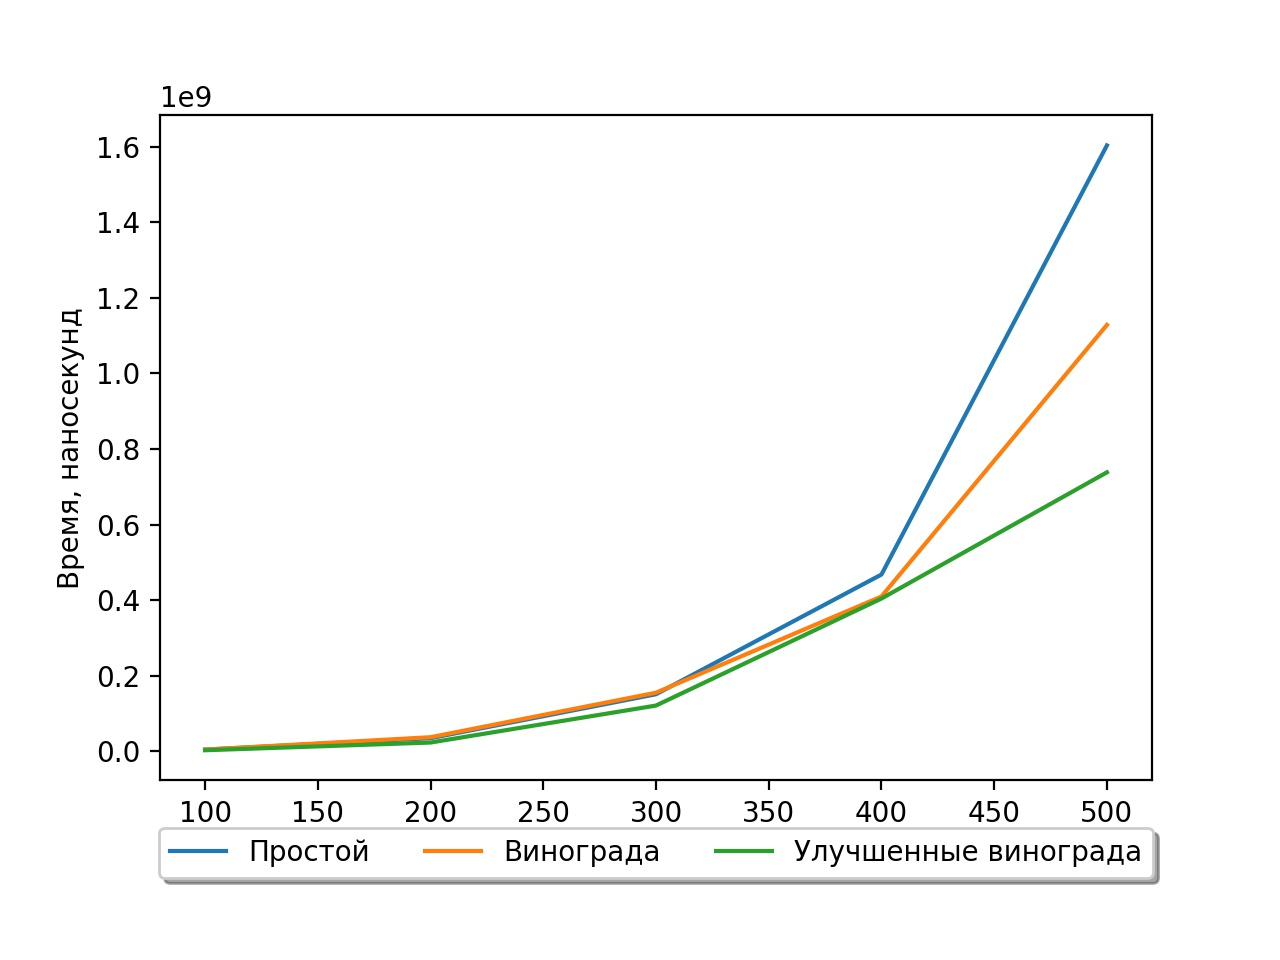
\includegraphics[]{sem-v-aa-master/lab1/tex/inc/plots/lab2_even.jpg}
    \caption{Временные характеристики для нечетных размеров матриц}
    \label{fig:even}
\end{figure}

\begin{figure}
    \centering
    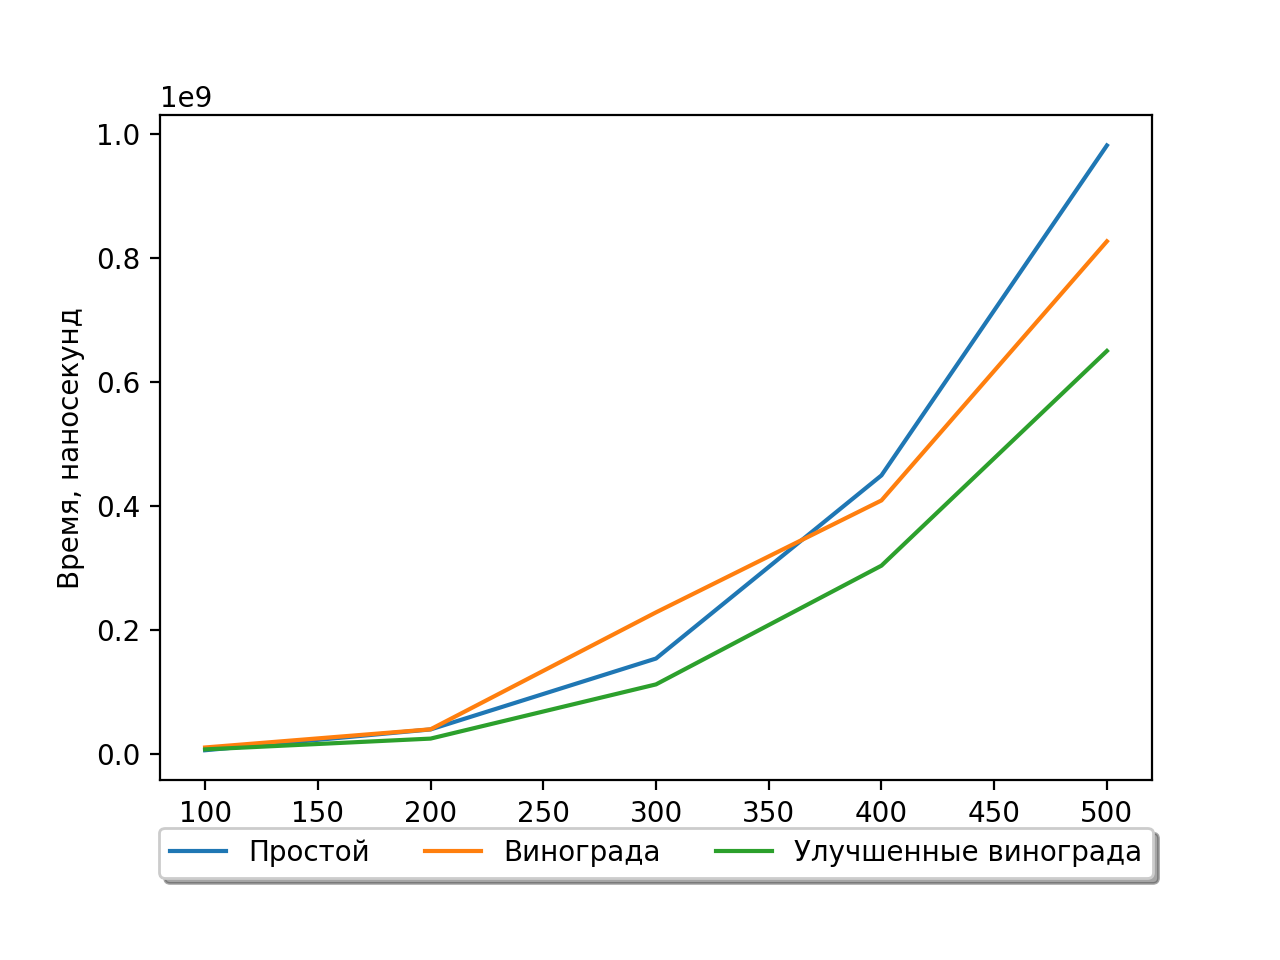
\includegraphics[]{sem-v-aa-master/lab1/tex/inc/plots/lab2_odd.png}
    \caption{Временные характеристики для четных размеров матриц}
    \label{fig:odd}
\end{figure}

\section{Вывод}

В данном разделе было произведено сравнение затраченного времени для каждого из ранееизложенных алгоритмов. Как и ожидалось, наиболее эффективным оказался оптимизированные алгоритм Копперсмита---Винограда. Он, в свою очередь, при размерность матрицы равной 500 в 1.6 раза эффективнее неоптимизированного алгоритма Копперсмита---Виноградаи и в 2.6 раза эффективнее простого алгоритма. 

Не столь разительной оказалась разница между простым алгоритмом и неоптимизированного алгоритма Копперсмита---Винограда: последний имеет в полтора раза большую производительность.

Полученные характеристики для  матриц нечетных размерностей отличны от матриц четных размерностей, и в сравнении с последними показывают медианно худший резльтат, что как было сказано, ранее вызвано дополнительным условием на нечетность размеров матрицы. 

Таким образом, полученный экспериментально результат в целом совпадает с заранее вычисленным теоретически в аналитическом разделе. 

%%% Local Variables:
%%% mode: latex
%%% TeX-master: "rpz"
%%% End:
